\documentclass[acmplain,acmnow]{acmtrans2m}

%\newtheorem{theorem}{Theorem}[section]
%\newtheorem{conjecture}[theorem]{Conjecture}
%\newtheorem{corollary}[theorem]{Corollary}
%\newtheorem{proposition}[theorem]{Proposition}
%\newtheorem{lemma}[theorem]{Lemma}
%\newdef{definition}[theorem]{Definition}
%\newdef{remark}[theorem]{Remark}

\usepackage[dvips]{color}
\usepackage{graphicx}

\title{Exploring Android Stack by implementing a complete flow, from Java application layer to native library}
            
\author{ANTONIO TROINA\\
		{\small M. 708267 (antonio.troina@mail.polimi.it)}\\
		{\footnotesize Dipartimento di Elettronica e Informazione, Politecnico di Milano, Milan, IT}}
            
\begin{abstract} 
This paper aims to briefly analyze Android internal architecture, and to describe, through a convienient and properly documented example, the necessary steps to break into the Android stack, and implement a customised native daemon - which relies on its own native library - that can communicate with a Java application through the Java Native Interface.\\
The first part of this work will cover the Android stack, with a general overview of its main components, while the second part will propose a basic implementation of a client-server paradigm, whose actors will be a Java-coded app (client) and a C-coded daemon (server).
\end{abstract}
            
\category{D.4.7}{Real-time systems and embedded systems}{Android}
\keywords{Android, JNI}  
\begin{document}
\maketitle

\newpage
\markright{Contents}
\tableofcontents
\vskip\baselineskip%
\begin{center}
\line(1,0){250}
\end{center}
\vskip\baselineskip%
\listoffigures
%\thispagestyle{empty}
%\mbox{}

\markright{Introduction}

\section{Introduction}
In 2011, 48.8\% of the smartphones on the market, ran Android OS, contributing to an annual growth of 244\%.\footnote{Source: Canalys. February 2012} This is what an average customer can easily guess by himself. What not everyone can figure, unless he's working in this very specific field, is that lately Android OS - and therefore its open source project AOSP - aroused the curiosity of many embedded developers. Despite not being as "lightweight and small footprint"-centric as other \textit{Real Time Operating System}, Android still offers a lot of opportunities to Embedded Developers: first of all, a very intuitive graphic interface. While a large number of embedded devices have little to no human interface, a substantial number of devices which would traditionally be considered "embedded" do have user interfaces. In this field, Android comes as a bridge connecting the users that are already familiar with its interface, to embedded systems they need to interact with.\\
Despite in the past common GUI were window-centric and desktop-like, after iOS and Android birth the way people interact with mobile instruments and devices has changed, towards a more touch-based experience. This change, combined with Android's open source licensing, has been a terrific mix that increased embedded developers' interest in Android open source project.\\
This work will analyse Android's structure, to better understand the whole flow which goes from Java App (which is called Activity) to the native code, running below anything, and just above the kernel. All this will be done through a very simple example, where a native daemon running throughout the whole Android's execution will be able to grant some dummy resources (we called cores) to a Java application requiring them. This communication will go through the whole stack in a top down approach relying on JNI interface. A small bottom up example which uses a \textit{callback} function will be presented as well.
\markright{Android Internals}
\section{Android Internals - Overview}
\label{overview}
As we can see in Fig. \ref{fig:stack} \cite{remixingand}, Android's architecture can be divided into many components, which we'll briefly analyse - following a bottom-up approach - before going deeper into the core of this work.
\begin{figure}[!htb]
	\centering
	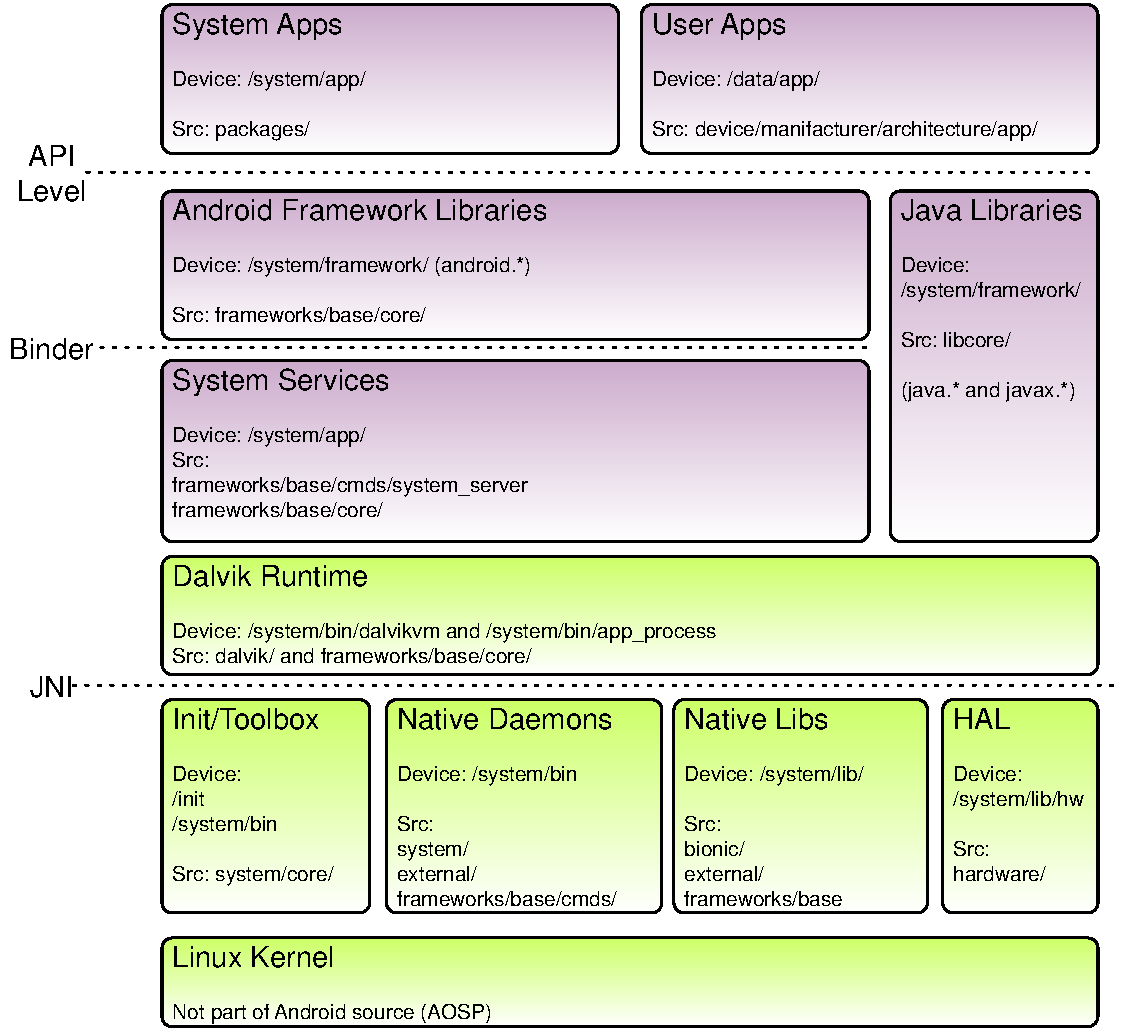
\includegraphics[scale=.6]{images/stack.pdf}
	\caption{Android's stack}
	\label{fig:stack}
\end{figure}
\begin{itemize}
\item \textbf{Linux Kernel}\\
Android kernels are, in sum, forks from the mainline kernel, relying on several custom 	functionalities that are significantly different from what is found in the "vanilla" kernel. Follows a brief enumeration of the most remarkable customizations made to the kernel to satisfy special Android's needs.
	\begin{itemize}
	\item \textsc{Wakelocks}\\
	Instead of letting the system be put to sleep at the user's behest, an "Androidized"
kernel is made to go to sleep as soon and as often as possible. \textit{Wakelocks} are provided to keep the system awake while performing specific processing. The wakelocks and early suspend functionality are actually built on top of Linux's existing power management functionality.
	\item \textsc{Low Memory Killer (Viking Killer)}\\
	Since Android system typically runs in low-memory conditions, the \textit{out-of-memory} (OOM) handling is crucial: therefore the Android development team has introduced an additional \textit{LMK} - based on priorities to identify \textit{to-be-killed} candidates - that kicks in just before the default kernel OOM killer does (thus preempting its intervention, which occurs only when no memory is left).
	\item \textsc{Binder}\\
	Binder allows apps to talk the System Server and it's what apps use to talk to each others' service components, although they actually perform this communication through  interfaces and stubs generated by the \textit{aidl} tool. In Fig. \ref{fig:binder_flow} and example of the communication flow: the Activity (which is what we're used to call "App", despite this word in the Android Framework acquires different meanings) requires to the \textit{Service Manager} an instance of a specific Service she wants to interact with, and performs this operation through \textit{Stubs} and \textit{Binder}.
		\begin{figure}[!htb]
			\centering
			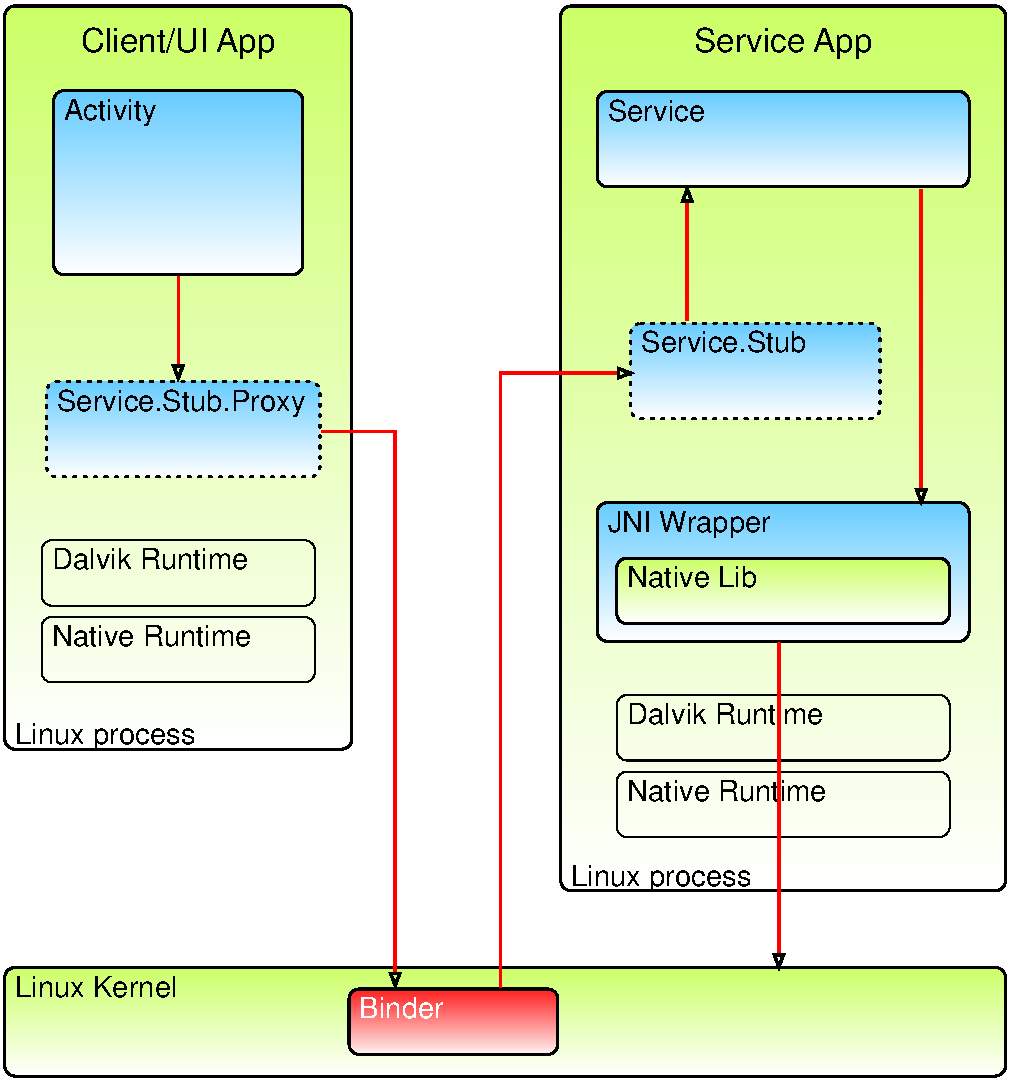
\includegraphics[scale=.4]{images/binder_flow.pdf}
			\caption{Communication Activity-Service through Binder}
			\label{fig:binder_flow}
		\end{figure}
	\item \textsc{Anonymous Shared Memory}\\
	Typically, a first process creates a shared memory region using \textit{ashmem} and uses Binder to share the corresponding file descriptor with other processes with which it wishes to share the region. \textit{Ashmem} destroys memory regions when all processes referring to them have exited and will shrink mapped regions if the system is in need of memory.
	\item \textsc{Alarm}\\
	Android's alarm driver is actually layered on top of the kernel's existing Real-Time Clock (RTC) and High-Resolution Timers (HRT) functionalities. Android's alarm driver cleverly combines the best of both worlds: by default the driver uses the kernel's High-Resolution Timer (HRT) functionality, but whenever the system is about to suspend itself, it programs the RTC so that the system gets woken up at the appropriate time.
	\item \textsc{Logger}\\
	Android defines its own logging mechanisms based on the Android logger driver added to the kernel. The lightweight Android Logger manages a handful of separate kernel-hosted buffers for logging data coming from user-space. The driver maintains circular buffers where it logs every incoming event and returns immediately back to the caller.
	\end{itemize}
So far the most evident kernel customisations have been described, despite they are actually more, nonetheless a deeper analysis of the Android kernel is out of the scope of this document.
\item \textbf{Hardware Abstraction Layer [HAL]}\\
Keeping in mind Fig. \ref{fig:stack}, let's examine the HAL module. The Android stack typically relies on shared libraries provided by manufacturers to interact with hardware. In effect, Android relies on what can be considered a Hardware Abstraction Layer (HAL), and we can mainly identify the following advantages:
	\begin{itemize}
		\item Separates Android platform logic from specific hardware interfaces
		\item User­space HAL offers standard "driver" definitions for graphics, audio, camera, bluetooth, GPS, radio (RIL), WiFi, etc.
		\item Makes porting easier
		\item Other - minor - license-related reasons
	\end{itemize}
\begin{figure}[!htb]
	\centering
	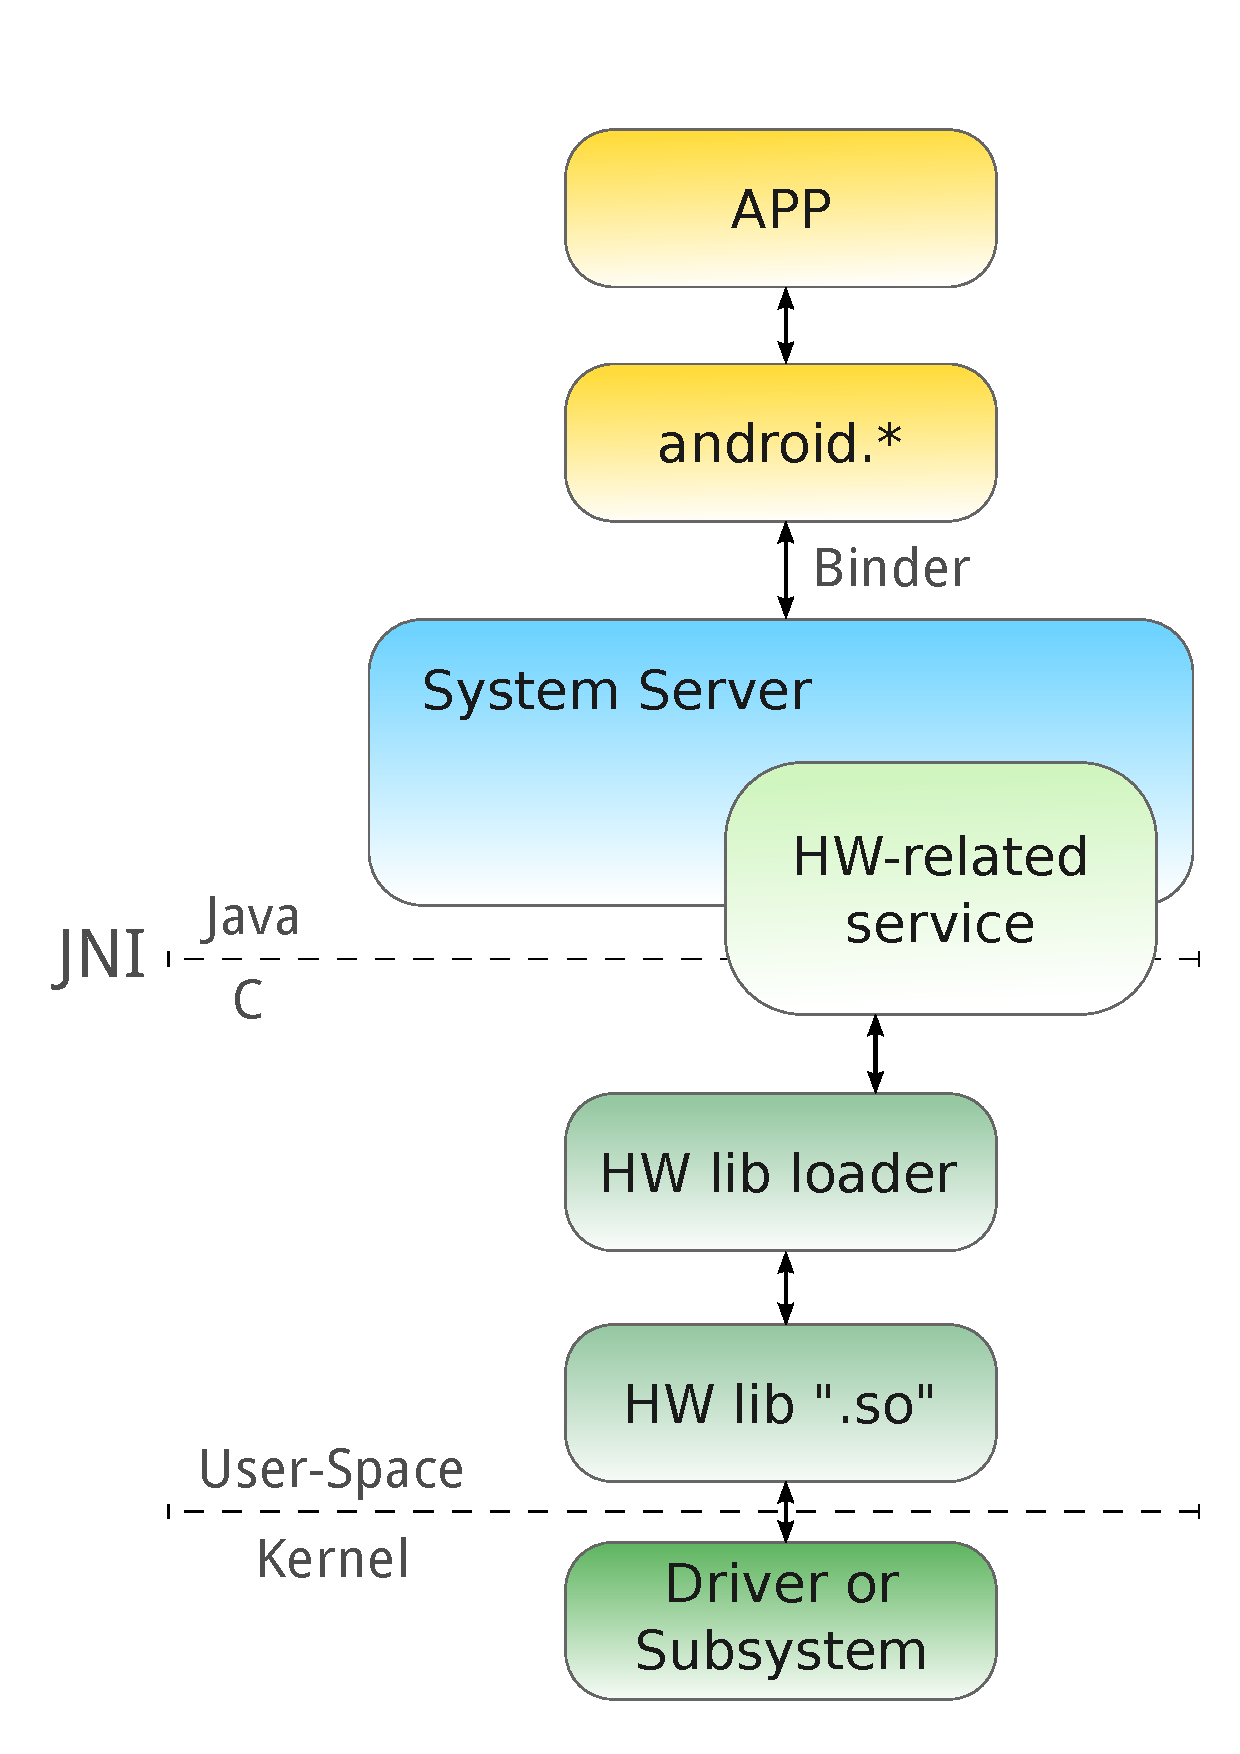
\includegraphics[scale=.25]{images/hal.pdf}
	\caption{Hardware Abstraction Layer structure}
	\label{fig:hal}
\end{figure}
A typical example of the way in which Android abstracts and supports hardware can be seen in Fig. \ref{fig:hal}: it's easy to notice that the hardware support outside the bare Kernel is substantial. As a consequence, Android, to run on a specific hardware, requires more than just a proper driver: a hardware module (not a kernel module) which conforms to the API specified for that type of hardware, must be provided.
\item \textbf{Native Libraries}\\
Android relies on slightly more than a hundred dynamically-loaded libraries (in our testing configuration, 124), which are stored in /system/lib. The largest part of them is actually generated within the AOSP, and a portion comes from external projects, merged into AOSP codebase to add some specific functionalities.
\item \textbf{Native Daemons}\\
As already seen into Linux, Android typically runs some \textit{Daemons}, which are native processes - launched at startup phase, or when expressly requested - that continue to run throughout the lifetime of the system.
\item \textbf{Init}\\
The list of automatically launched daemons during the startup phase (with permission and other options) can be found in \textit{init.rc} file: \textit{\textbf{init}} - as happens into Linux - is the first process started immediately after the Linux boot, and \textit{init.rc} is its configuration file.
\item \textbf{Dalvik VM}\\
Long story short: Dalvik VM is Android's Java Virtual Machine, with a substantial difference, as shown in Fig. \ref{fig:dalvik}, and after written.\\
\begin{figure}[!htb]
	\centering
	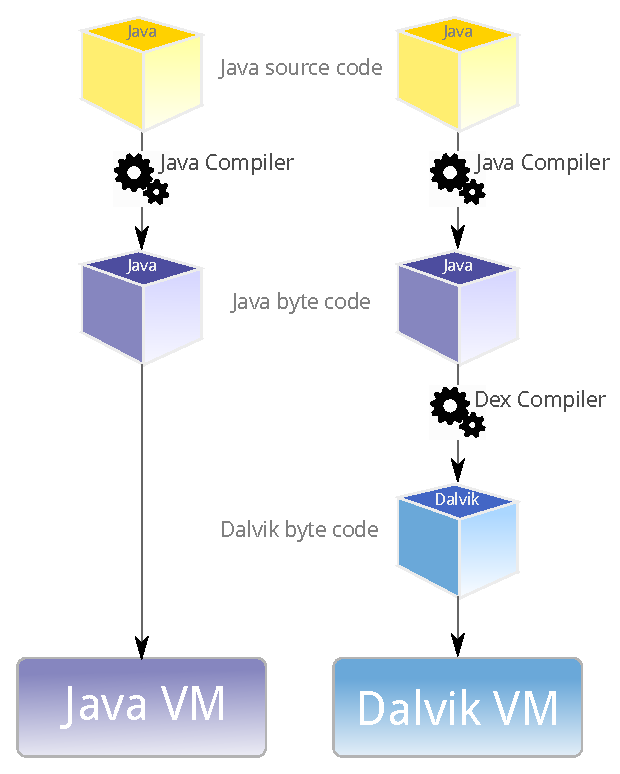
\includegraphics[scale=.7]{images/dalvik.pdf}
	\caption{Comparison Java - Dalvik}
	\label{fig:dalvik}
\end{figure}
While in Java the source code is compiled into Java byte code, which can run on the Java VM, in Android there's one more halfway step, which passes through the \textit{dx utility}, which is a \textit{Dex compiler}: \textit{.dex} files, created by postprocessing the \textit{.class} files generated by the Java compiler - when uncompressed are 50\% smaller than their originating .jar files - can finally run on the Dalvik VM which therefore can't straight run Java byte code.
\definecolor{lightgray}{gray}{0.93}
  \vskip\baselineskip%
  \par\noindent\colorbox{lightgray}{%
    \begin{minipage}{0.953\textwidth}
		\textsc{Good to know}:\\
		In 2010 an interesting feature of Dalvik has been introduced: a Just-In-Time (JIT) compiler for ARM. This compiler allows \textit{.dex} byte code files to be converted to binary assembly instructions that run natively on the target's CPU (only ARM so far) instead of being interpreted one instruction at a time by the VM. The first time you load the app it may take a bit longer, but once an App has been \textit{"JIT-ed"}, then it loads and runs much faster than being interpreted.
    \end{minipage}%
  }%
  \vskip\baselineskip%
\end{itemize}
Before we go on analysing the \textit{System Services} block (again, Fig. \ref{fig:stack}), it's worth focusing on JNI interface, which basically permits the communication between the \textit{Java} world and the \textit{Native} one.
\begin{itemize}
\item \textbf{Java Native Interface [JNI]}\\
Java written code sometimes needs to interface to native code written in C/C++, and this sentence comes especially true in the embedded systems' world: in fact, to access to low-level functionalities, Java applications need to interact with native daemons and libraries. This bridge role is played by what is known as \textit{Java Native Interface}.\\
JNI allows programmers to take advantage of the power of the Java platform, without having to abandon their investments in legacy code: this means also that you can port your C/C++ code to Android with a bit of investment on implementing a sort of \textit{"glue code"} which lets Android applications using it. JNI has been defined as \textit{"a dark art reserved to the initiated"} \cite{embandroid} therefore, for the time being, it's enough to have an idea of what it is.
\item \textbf{System Services}\\
System services (e.g. Location service, Sensor service, WiFi service, Alarm service, Telephony service, Bluetooth service, and so on) are always on, always running, and readily available for developers to tap into, started at boot time and are guaranteed to be running by the time your application launches. They cooperate together through Binder, the mechanism on which all system services are built.\\
System services are basically divided in two parts: mainly Java-coded services (but two), running under the \textit{system server} process, and C/C++ coded services, running under the \textit{media server} process.\\
As we did for JNI, we won't go deeper into the details of System Services now, although we'll better understand its functioning theough an example. Fully understanding the internals of Android's system services has been defined as \textit{trying to swallow a whale} \cite{embandroid}.
\item \textbf{Service Manager}\\
As the director of orchestra, the Service Manager coordinates all the system services, and allows Android Applications to access System Services: as we'll see in the second part of this work, an Application can invoke the
\begin{verbatim}
	serviceManager.getSystemService(SERVICE_NAME);
\end{verbatim} method on the ServiceManager object. This interaction nevertheless isn't as simple as it could seem at first sight, since the whole process uses the Binder paradigm. (Figg. \ref{fig:service_manager} and \ref{fig:binder_flow}) despite Android Development Team made all this quite transparent to the Application developer, who typically doesn't need to implement his own service, but just to use the ones already built by AOSP.
\begin{figure}[!htb]
	\centering
	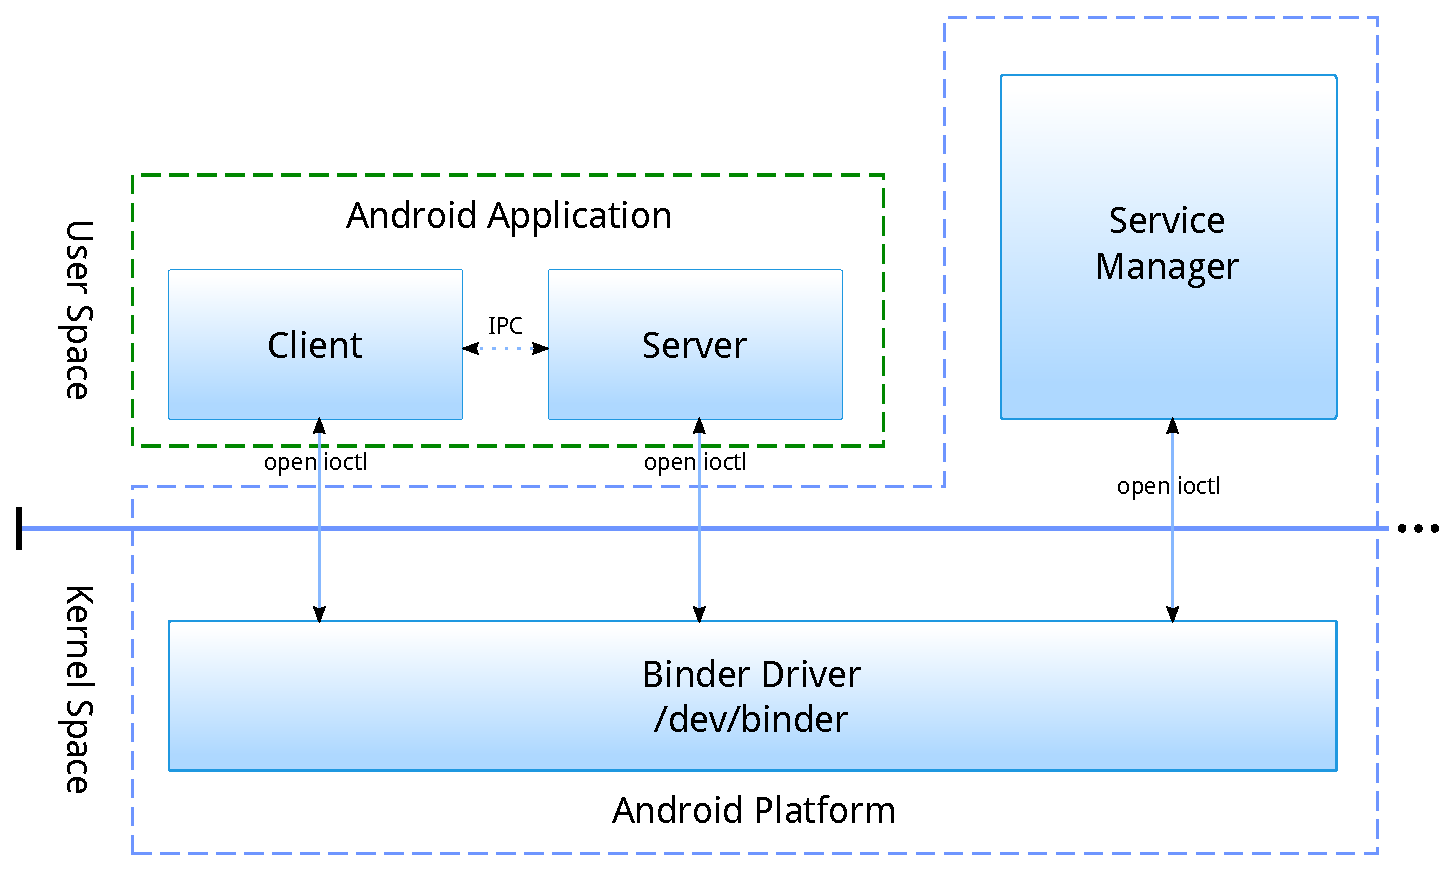
\includegraphics[scale=.5]{images/service_manager.pdf}
	\caption{Interaction "Application - Service manager", through Binder}
	\label{fig:service_manager}
\end{figure}
\item \textbf{Android Framework Libraries}\\
Libraries that allow the Application, through Java Interfaces, to access the proper native libraries: whenever an instance of a library class is created, a call to the ServiceManager - through binder - is made, to get the proper Service (or System Service) as Interface (binded to an .aidl file), which finally permits the Application to call Java libraries' methods that, through JNI, are connected to the native library.
\end{itemize}
The higher level isn't that much of our interest for this work, as it includes the "Apps" layer, which actually are called "Activities", and they are just the presentation level of the whole stack. Nevertheless we will see in the last part of this work (Section \ref{Customising}.) the implementation of a very simple Activity to graphically interact with our custom native daemon.
\markright{Environment setup}
\section{Environment setup}
\label{setup}
Basically, to have a foundation we can work on, a ready-to-run AOSP system should be setup and properly configured. The most important instructions can be found at the AOSP project website: \texttt{http://source.android.com/}\\
In this section the basic steps will be presented, especially highlighting the main issues that have been encountered during the development.
\subsection{Initialize the build environment}
The on-line guide to initialize the system can be found at:\\
\texttt{http://source.android.com/source/initializing.html}\\
It is based on Ubuntu LTS (10.04), nevertheless the environment I used was Linux Mint 13, which is based on Ubuntu (12.04).\\
Leaving aside the default recommendations by the AOSP webpage, let's see what actually went wrong, and how to fix it:
\begin{itemize}
\item \textbf{Java Development Kit}\\
The android source suggests to install, among the others, the OpenJDK package:
	\begin{verbatim}
		$ sudo apt-get install openjdk-6-jdk
	\end{verbatim}
This didn't work, since I found out that Android 2.3+ requires Java 6 to build correctly. While OpenJDK did work for 2.3, it doesn't for Android 4.0: you need Sun Java Development Kit. A solution is to download the JDK 1.6 binary release from Sun's Java download site and unzip it somewhere in your system, for example:
	\begin{verbatim}
		$ sudo mkdir -p /opt/java/64/
		$ sudo cp jdk-6u33-linux-x64.bin /opt/java/64
		$ sudo su -
		$ cd /opt/java/64
		$ chmod +x jdk-6u29-linux-x64.bin
		$ ./jdk-6u33-linux-x64.bin
		$ exit
	\end{verbatim}
Add the new Java to your shell environment's \texttt{\$PATH} so it takes priority over other Javas you might have installed (yes, this means that different JDK can coexist):
	\begin{verbatim}
		$ echo 'export PATH=/opt/java/64/jdk1.6.0_33/bin:$PATH' \
		       >> ~/.bashrc
	\end{verbatim}
If you relaunch your terminal (do it) you should be able to see the change with the command \texttt{java -version}
\item \textbf{GCC - The Gnu Compiler Collection}\\
By default I found on my system the latest version of the \texttt{gcc} compiler, which - at the time of this writing - is the \texttt{4.6}: this version works smoothly with Android Jelly Bean, but presented some fatal errors which didn't let me complete the compilation on Icecream Sandwich. A solution - for the latter - has been to install the \texttt{4.4} version (as for JDK, two different versions can coexist on the same system).
	\begin{verbatim}
		$ sudo apt-get install gcc-4.4 g++-4.4 \
		                       g++-4.4-multilib gcc-4.4-multilib
	\end{verbatim}
This works, with the watchfulness of explicitly declare you want to use this specific gcc version at compile time, by passing it as argument to the make command, as follows:
\definecolor{lightgray}{gray}{0.93}
  \vskip\baselineskip%
  \par\noindent\colorbox{lightgray}{%
    \begin{minipage}{0.953\textwidth}
		\textsc{Remember}:\\
			\texttt{\$ make CC=gcc-4.4 CXX=g++-4.4 -j8}
    \end{minipage}%
  }%
  \vskip\baselineskip%
I put stress on this because I'm sure it can save you time, and prevent you from banging the desktop with your forehead, in case you're building an older version of Android.\\
The \texttt{-j8} option tells the compiler to launch 8 parallel threads, therefore if you are compiling on a multi-core architecture, this may save you quite a lot of time: you can choose the value that better fits your cpu architecture.
\item \textbf{Libraries}\\
Since I built and installed other packages during my work, I experienced that the most commonly replaced ones were:
	\begin{itemize}
		\item libncurses5-dev:i386
		\item libgl1-mesa-glx:i386\\
		For this one is convenient to do this:
		\begin{verbatim}
			$ sudo ln -s /usr/lib/i386-linux-gnu/mesa/libGL.so.1 \
			             /usr/lib/i386-linux-gnu/libGL.so
		\end{verbatim}
	\end{itemize}
Therefore, if the compilation - that previously was working - suddenly doesn't work anymore, check whether you still have those two libraries and their versions.
\end{itemize}
Last suggestion, as the AOSP website says, it's recommended enabling the \texttt{CCACHE} option, to save time during the following compilations. You can do it by executing the following bash command:
\begin{verbatim}
$ export USE_CCACHE=1
\end{verbatim}
\subsection{Downloading the source tree}
All instructions to download the source files can be found at this address:\\
\texttt{http://source.android.com/source/downloading.html}
\subsection{Building the system}
All instructions to build the system can be found at this address:\\
\texttt{http://source.android.com/source/building.html}
\markright{System setup}
\section{System setup}
\label{Customising}
This work, as stated in the abstract, aims to implement a native daemon (constantly running) which will be exposed as a System Service to the Java application layer. The Java application will be able to communicate with the daemon through JNI and the native library, and the other way around will be implemented by using a callback function.\\
Since this project is focused on understanding the basics of Android, to afterwards integrate a native RTRM application as a System Service - therefore accessible by the Java environment - I decided to implement this simple daemon as a dummy-RTRM which will communicate with the application the number of available "cores" (actually will be just an \texttt{int}) and allow it to "require" or "release" cores (with a sort of \texttt{core++} and \texttt{core--} functions).
\subsection{Setting up the directory structure}
The followed approach has been to keep separate the main code from our customised code, so that our platform-specific code will be compiled when the user will choose to build our specific system, instead of the default one. This choice results in a more atomic and modular way to operate.\\
In the \texttt{aosp} directory, there's a folder named \texttt{device}, which typically contains folders indicating manifacturers, and into each manifacturer's folder, the specific architecture folder: in our case, the manifacturer folder has been named \texttt{bosp}, and the architecture folder \texttt{p2012}. To properly organize files, we have a main \texttt{p2012} folder, and a \texttt{p2012-common} folder, which contains the largest part of our customised code.
\begin{verbatim}
device/
├── bosp/
│   ├── p2012/
│   │   ├── app/
│   ├── p2012-common/
│   │   ├── app/
│   │   ├── bin/
│   │   ├── framework/
│   │   └── lib/
\end{verbatim}
Let's briefly see what these folders contain:
\begin{itemize}
	\item \texttt{p2012/app}: contains configuration files to identify the board, the architecture, the packages that will be built-in with this version, and the possible "Activities" that will be coded especially for this release.
	\item \texttt{p2012-common/app}: contains the Java code of the \texttt{ServiceApp} that will register our new service to the \textit{Service Manager} as a remote service, through the call
	\begin{verbatim}
		ServiceManager.addService(REMOTE_SERVICE_NAME, this.serviceImpl);
	\end{verbatim}
	\item \texttt{p2012-common/bin}: contains the C/C++ code of the \textit{native daemon}. Once exported as local module, its name will be added to the \texttt{init.rc} file, to let it start at bootup stage.
\definecolor{lightgray}{gray}{0.93}
  \vskip\baselineskip%
  \par\noindent\colorbox{lightgray}{%
    \begin{minipage}{0.953\textwidth}
		\textsc{Good to know}:\\
		Any C/C++ source put into this folder (along with the proper \texttt{Android.mk} configuration file - see Section \ref{build-system}), will be compiled by Android's building system as a module, and put into device's \texttt{/system/bin} folder, so that will be ready to run within the environment.
    \end{minipage}%
  }%
  \vskip\baselineskip%
	\item \texttt{p2012-common/framework}: contains two main folders, one includes the whole JNI-related stuff (both C/C++ and Java sources), and the other one comprises the Java source of our specific-service Manager class (which handles the Binding procedure, once created) and the \texttt{.aidl} file, which basically is an interface.
	\item \texttt{p2012-common/lib}: contains the C/C++ source code for our specific libraries and headers.
\end{itemize}
Once we have this basic structure, we can go deeper into details of the configuration files needed by the \textit{make system}.
\subsection{Configuration files}
\label{configuration}
We are mainly operating inside the \texttt{p2012} folder so, unless specified, this will be our working directory for this section.
\begin{enumerate}
\item \label{item-and-vendors} At first, we create a file named \texttt{vendorsetup.sh}, which will contain the name of the \textit{lunch-combo} we want to associate to our new device. My file would look like this:
\begin{verbatim}
	add_lunch_combo full_bosp_p2012-eng
\end{verbatim}
where \texttt{full} indicates that we're starting, as base - from Android build with the most complete set of Application/Services, \texttt{bosp\_p2012} indicates our customised build, \texttt{eng} indicates the development configuration with additional debugging tools.\\
From within the main \texttt{aosp} directory, if you open a shell and launch the following
\begin{verbatim}
	$. build/envsetup.sh
\end{verbatim}
you should see the system including the new configuration.
\item \label{item-and-prod} The file \texttt{AndroidProducts.mk} contains the reference to the specific product build makefiles, therefore we indicate here this:
\begin{verbatim}
	PRODUCT_MAKEFILES := $(LOCAL_DIR)/full_p2012.mk
\end{verbatim}
\item \label{item-and-makefile} And here a piece of our \texttt{full\_p2012.mk} file
\begin{verbatim}
	$(call inherit-product, $(SRC_TARGET_DIR)/product/
	                        languages_full.mk)
	$(call inherit-product, $(SRC_TARGET_DIR)/product/full_base.mk)
	PRODUCT_NAME := full_p2012
	PRODUCT_DEVICE := p2012
	PRODUCT_MODEL := Full BBQUE P2012 Image for Emulator
	# Include the common definition and packages
	include $(LOCAL_PATH)/../p2012-common/bosp_p2012.mk
	include $(call all-makefiles-under,$(LOCAL_PATH))
\end{verbatim}
To our scope, to have a more lightweight build, we change \texttt{languages\_full.mk} and \texttt{full\_base.mk} respectively, with \texttt{languages\_small.mk} and \texttt{generic.mk}.\\
More "flavors" can be found into
\begin{verbatim}
	/aosp/build/target/product/
\end{verbatim}
\item Then we can copy/paste some basic configuration files from Android's main branch, in this way:
\begin{verbatim}
	$ cp build/target/board/generic/BoardConfig.mk \
	     device/bosp/p2012/.
	$ cp build/target/board/generic/AndroidBoard.mk \
	     device/bosp/p2012/.
	$ cp build/target/board/generic/device.mk \
	     device/bosp/p2012/.
	$ cp build/target/board/generic/system.prop \
	     device/bosp/p2012/.
\end{verbatim}
\item A further step for creating our own platform version, should be to generate platform signing keys, despite this is needed to pass \textit{Compatibility Test Suite}. At first, we create a local variable with our generalities:
\begin{verbatim}
	$ SIGNER="/C=IT/ST=Italy/L=Milan
	          /O=Polimi/OU=Android
	          /CN=Android Platform Signer
	          /emailAddress=john.doe@polimi.com"
\end{verbatim}
Then we generate keys with our signer details:
\begin{verbatim}
	$ echo | development/tools/make_key \
	         build/target/product/security/platform "$SIGNER"
\end{verbatim}
And run the same command three times more, replacing the \texttt{platform} word with: \texttt{shared}, \texttt{media}, \texttt{testkey}.\\
This step is required for the \textit{Compatibility Test Suite}.
\item We can now \textbf{build our own Android system}, which - so far - is just a simple \textit{Vanilla Android}. Any time you have to compile, be sure that you've run the following commands, in this order:
\begin{verbatim}
	$ . build/envsetup.sh
	$ lunch full_bosp_p2012-eng #here the build name you chose
	$ export USE_CCACHE=1
	$ make -j8
\end{verbatim}
\end{enumerate}
\definecolor{lightgray}{gray}{0.93}
  \vskip\baselineskip%
  \par\noindent\colorbox{lightgray}{%
    \begin{minipage}{0.98\textwidth}
		\textsc{Good to know}:\\
		At this point it's possible even to \textbf{customise the kernel}, nevertheless we don't need it. An example of the procedure to have it, can be easily found online.
    \end{minipage}%
  }%
  \vskip\baselineskip%
\subsubsection{Android build system}
\label{build-system}
Android build system mainly relies on a huge number of \textit{makefiles} named \textit{Android.mk}. Unlike Linux recursive make approach, Android's build system is based on the search of \texttt{Android.mk} files into any folder below the main one: whenever found - unless explicitly specified in the file - the search doesn't go any deeper. At the end of the process, all the information contained into those configuration files are summed up to a single file, which is the one used by the make process to compile each \textit{module} of the system. In Android's context, the word \textit{module} indicates any component of the AOSP that needs to be built. This might be a binary, an app package, a library, etc.\\
After typing \texttt{make} the system will hang up for a while with no output: during this time it's just assembling the final configuration file out of all the \texttt{Android.mk} files it has found.\\
Let's see how the configuration files should be organized inside our tree, to properly build:
\begin{verbatim}
├── p2012/
│   ├1── AndroidBoard.mk
│   ├2── AndroidProducts.mk
│   ├ ── app/
│   ├3── BoardConfig.mk
│   ├4── device.mk
│   ├5── full_p2012.mk
│   ├6── system.prop
│   └7── vendorsetup.sh
├── p2012-common/
│   ├ ── app/
│   ├ ── bin/
│   ├8── bosp_p2012.mk
│   ├ ── framework/
│   ├9── init.rc
│   └ ── lib/
\end{verbatim}
Files have been numbered to briefly explain their meaning (or, at least, what we do need to know concerning our work).
\begin{enumerate}
	\item[1,3,4,6] configuration files that we just copy/paste-d from the default branch, contain information about the device to emulate, used to set-up the building system.
	\item[2] reference to the main makefile (in our case, \texttt{full\_p2012.mk}) - see \ref{configuration} (\ref{item-and-prod})
	\item[5] Main makefile, contains an \texttt{include} directive to import other makefiles, and information about packages that will be built within the system-to-be - see \ref{configuration} (\ref{item-and-makefile})
	\item[7] see \ref{configuration} (\ref{item-and-vendors})
	\item[8] makefile which is local to the \texttt{p2012-common} folder. This is included by \texttt{5}, as being appended
	\item[9] we are going to see later what this file will contain, but basically we just need it to launch our native daemon during the startup phase.
\end{enumerate}
More detailed information about build system can be found into a file contained in AOSP directory: \texttt{build/core/build-system.html}\\
Now we set-up the system, we can start the implementation of our code.
\markright{Implementation}
\section{Implementation}
\label{Implementation}
\definecolor{lightgray}{gray}{0.93}
  \vskip\baselineskip%
  \par\noindent\colorbox{lightgray}{%
    \begin{minipage}{0.98\textwidth}
		\textsc{Source Code}:\\
		The extended and working version of the code presented in this paper can be found on:\\
		\texttt{https://github.com/thoeni/rtos-project.git}
		\\At the time of this writing, there are three branches, the \texttt{main}, the \texttt{icecream} (which has been tested on \texttt{Android 4.0.1\_r1} and the \texttt{jb-callback} which includes the callback from C to Java.)
    \end{minipage}%
  }%
  \vskip\baselineskip%
As shortly described in the previous section, this small example relies on a native library we'll implement, and a summary of the flow from the Client Application (Activity named BbqueActivity) to the Server (Daemon named bbqued) can be seen in Fig.\ref{fig:projectoverview}.\\
\begin{figure}[!htb]
	\centering
	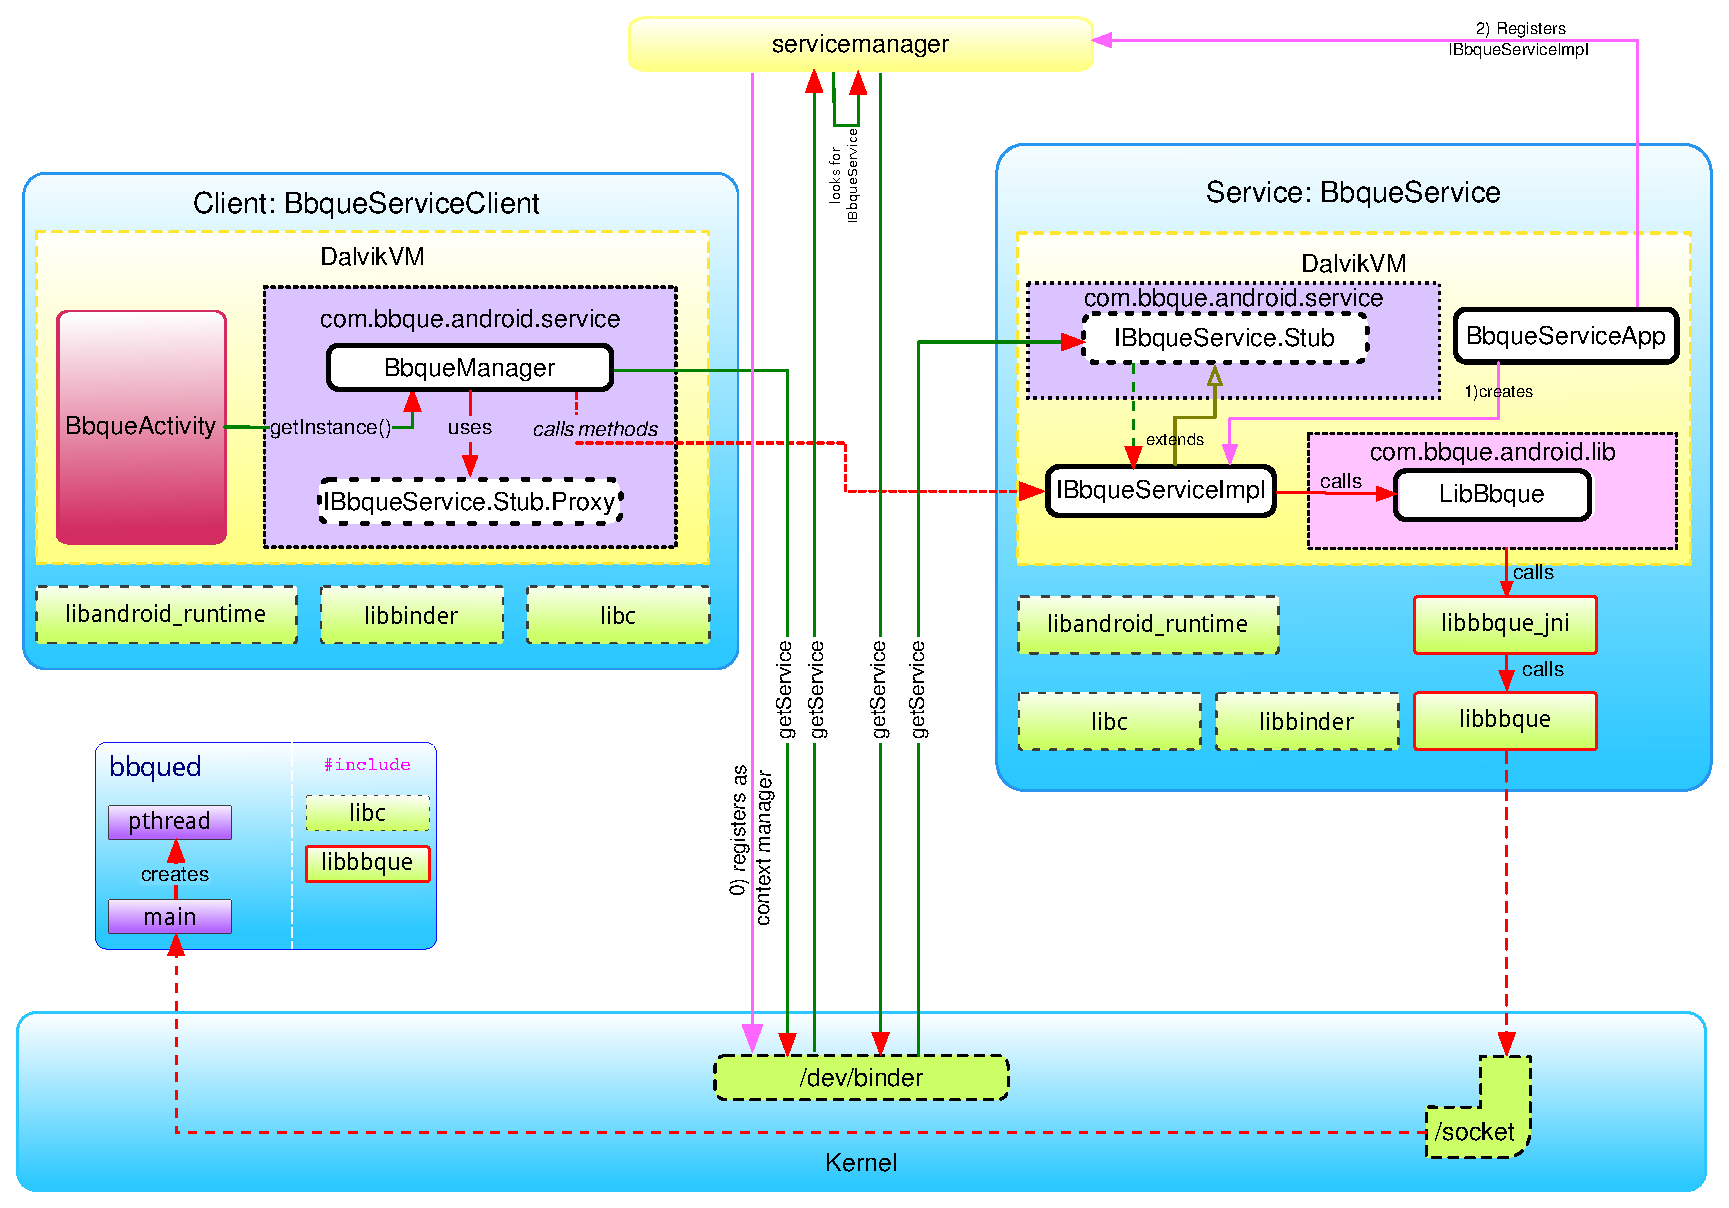
\includegraphics[scale=.432]{images/project_overview.pdf}
	\caption{Project flow overview}
	\label{fig:projectoverview}
\end{figure}
As a very high-level consideration, the modules on a \textbf{light blue} background run natively, while the modules over a \textbf{yellow} background run under Dalvik (therefore Java-coded). The \textbf{green} boxes are libraries, and the ones with a red stroke are included by our project. The \textbf{lilac} boxes are the two parts of our service, that communicate each other through binder. The \textbf{pink} box represents the Java module corresponding to our native library: the glue between them comes from JNI code. The flow indicated by the numbered \textbf{pink arrows} is executed during the startup phase.
\subsection{Native library}
Working directory for native library is \texttt{device/bosp/p2012-common/lib}.
The source tree for this directory is
\begin{verbatim}
lib/
|---Android.mk
|---libbbque/
    |---Android.mk
    |---libbbque.c
    |---libbbque.h
\end{verbatim}
The outermost \texttt{Android.mk} file contains just the instruction - for the building system - to search deeper for other \textit{makefiles}
\begin{verbatim}
	include $(call all-subdir-makefiles)
\end{verbatim}
The \texttt{libbbque} folder contains the \texttt{.h} header source with library's methods, \texttt{.c} source with library's methods implementation, along with another \texttt{Android.mk} file, which tells the building system how to build this library module (eg. indicates the source file, the shared libraries to include, the name of the module, its optionality, and so on).\\
For the sake of clarity, we'll consider as example the
\begin{verbatim}
extern int get_core_availability() {
   [...]
   send_message_to_bbqued ("core", &core_number);
   return core_number;
}
\end{verbatim}
the inner method connects to the \texttt{bbqued} daemon through a socket, and sends his message, for instance the string \texttt{"core"}, saving the server's response into \texttt{int core\_number} variable.\\
To register the library module to the system, so that we can - natively - access to it, it's necessary to add to the \texttt{/p2012-common/bosp\_p2012.mk} the following line:
\begin{verbatim}
[...]
PRODUCT_PACKAGES += libbbque
\end{verbatim}
This line will append to the list of other \texttt{PRODUCT\_PACKAGES} string, our customised module, that will be added to the build-to-be version of Android.\\
The library can now be built, potentially as a stand-alone make operation, as follows:
\begin{verbatim}
$ . build/envsetup.sh
$ lunch full_bosp_p2012-eng
$ export USE_CCACHE=1
$ make -j8 libbbque
\end{verbatim}
\subsection{Native daemon}
Working directory for native daemon is \texttt{device/bosp/p2012-common/bin}.
\begin{verbatim}
bin/
|---Android.mk
|---bbqued/
|   |---Android.mk
|   |---bbqued.c
\end{verbatim}
The outermost \texttt{Android.mk} file is identical to the \texttt{lib/} case, while the inner one contains instructions to properly build the daemon module.\\
The \texttt{bbqued.c} file, which imports the \texttt{libbque.h} library, implements the server side of our test, which creates a \textit{socket} and waits for any incoming connection. When a connection is received, it launches a thread (implemented by using \texttt{pthread} library): each thread reads/writes an \texttt{int} variable which is local to the main process. As done for the library, the daemon module must be added to the \texttt{/p2012-common/bosp\_p2012.mk} file:
\begin{verbatim}
[...]
PRODUCT_PACKAGES += bbqued
\end{verbatim}
\definecolor{lightgray}{gray}{0.93}
  \par\noindent\colorbox{lightgray}{%
    \begin{minipage}{0.98\textwidth}
		\textsc{Adding the process to} \texttt{init.d}:\\
		After building the system, will be possible to run the daemon by accessing the system through \texttt{adb shell} command, and running the \texttt{bbqued} command (since it will be placed straight into \texttt{/bin} folder.\\
		If you want your process to be started at system startup, you can add it to the \texttt{init.d} file that you should have copied before as follows
		\vskip\baselineskip%
		\texttt{\$ cp system/core/rootdir/init.rc device/bosp/p2012-common/.}
		\vskip\baselineskip%	
		Then the building system must be notified to copy this customised file to the target \texttt{root} directory, as follows:
		\vskip\baselineskip%		
		\texttt{PRODUCT\_COPY\_FILES += \$(MY\_PATH)/init.rc:root/init.rc}
    \end{minipage}%
  }%
  \vskip\baselineskip%
To build this module, we have to make the system, as usual.
\subsection{Wrapping native library with JNI}
\label{JNIwrapping}
JNI is the glue to let C and Java talking to each other. This code will be put into directory \texttt{/p2012-common/framework/}, divided int two sub-directories as follows:
\begin{verbatim}
bbque_jni/
|---Android.mk
|---java/
|   |---Android.mk
|   |---com/
|   |   |---bbque/
|   |       |---android/
|   |           |---lib/
|   |               |---LibBbqueException.java
|   |               |---LibBbque.java
|   |---com.bbque.android.lib.xml
|---jni/
    |---Android.mk
    |---com_bbque_android_lib_LibBbque.c
    |---com_bbque_android_lib_LibBbque.h
\end{verbatim}
Create the \texttt{LibBbque.java} class, which contains just the declarations of the methods we want to expose to Java world (which must be declared as \texttt{public native}), as follows:
\begin{verbatim}
public native static int getNumCore() throws LibBbqueException;
\end{verbatim}
and the declaration of the jni library:
\begin{verbatim}
static {
   System.loadLibrary("bbque_jni");
}
\end{verbatim}
The \texttt{xml} file contains the declaration of permissions for the library, that will be generated as \texttt{jar} file during the next step:
\begin{verbatim}
<library name="com.bbque.android.lib"
    file="/system/framework/com.bbque.android.lib.jar"/>
\end{verbatim}
And finally the \texttt{Android.mk} file, under \texttt{java/} directory, which is quite elaborate, states all the instructions to properly compile the whole module that will be therefore included into the build process.\\
Then, the \texttt{make} command will process the module, and will generate a jar file (tipically \texttt{classes-full-debug.jar}), which is needed by the next step, as input parameter to the \texttt{javah -jni} command, that generates the JNI header file.
\begin{verbatim}
$ javah -jni \
        -d device/bosp/p2012-common/framework/bbque_jni/jni/ \
        -classpath out/target/common/obj/JAVA_LIBRARIES/\ 
        com.bbque.android.lib_intermediates/classes-full-debug.jar \
        com.bbque.android.lib.LibBbque
\end{verbatim}
The first line suggests where the output header file will be placed, the second line gives as input the jar shared library generated during the previous step.\\
An example of an auto-generated signature, within the header file, is
\begin{verbatim}
JNIEXPORT jint JNICALL Java_com_bbque_android_lib_LiBbque_getNumCore
  (JNIEnv *, jclass);
\end{verbatim}
The next step consists into the implementation of the header file just generated, for example as follows:
\begin{verbatim}
JNIEXPORT jint JNICALL Java_com_bbque_android_lib_LiBbque_getNumCore
  (JNIEnv *env, jclass clazz) {
  jint result = get_core_availability();
  [...]
  }
\end{verbatim}
It's easy to realize that this is just a wrapping of the C native library.\\
After properly compiling the usual configuration files, \texttt{Android.mk} and the main \textit{makefile} \texttt{bosp\_p2012.mk} with the new modules to include, the system can be built again, and the native library is now accessible through \texttt{LibBbque} class:
\begin{verbatim}
LibBbque.getNumCore();
\end{verbatim}
We can say that the java call, so far, works within the upper right part of Fig.\ref{fig:projectoverview}, by calling Java methods on the \texttt{LibBbque} class (pink box).
\subsection{Binding the library with the Interface}
To let application-layer activities use the Java library previously created, an interface should be created, which will access to the library through \textit{Binder's} help.\\
To have an idea of the part of the flow in Fig.\ref{fig:projectoverview} we are working to, consider the greyed-out red-dashed-stroked area in Fig.\ref{fig:projectoverview_binder}.
\begin{figure}[!htb]
	\centering
	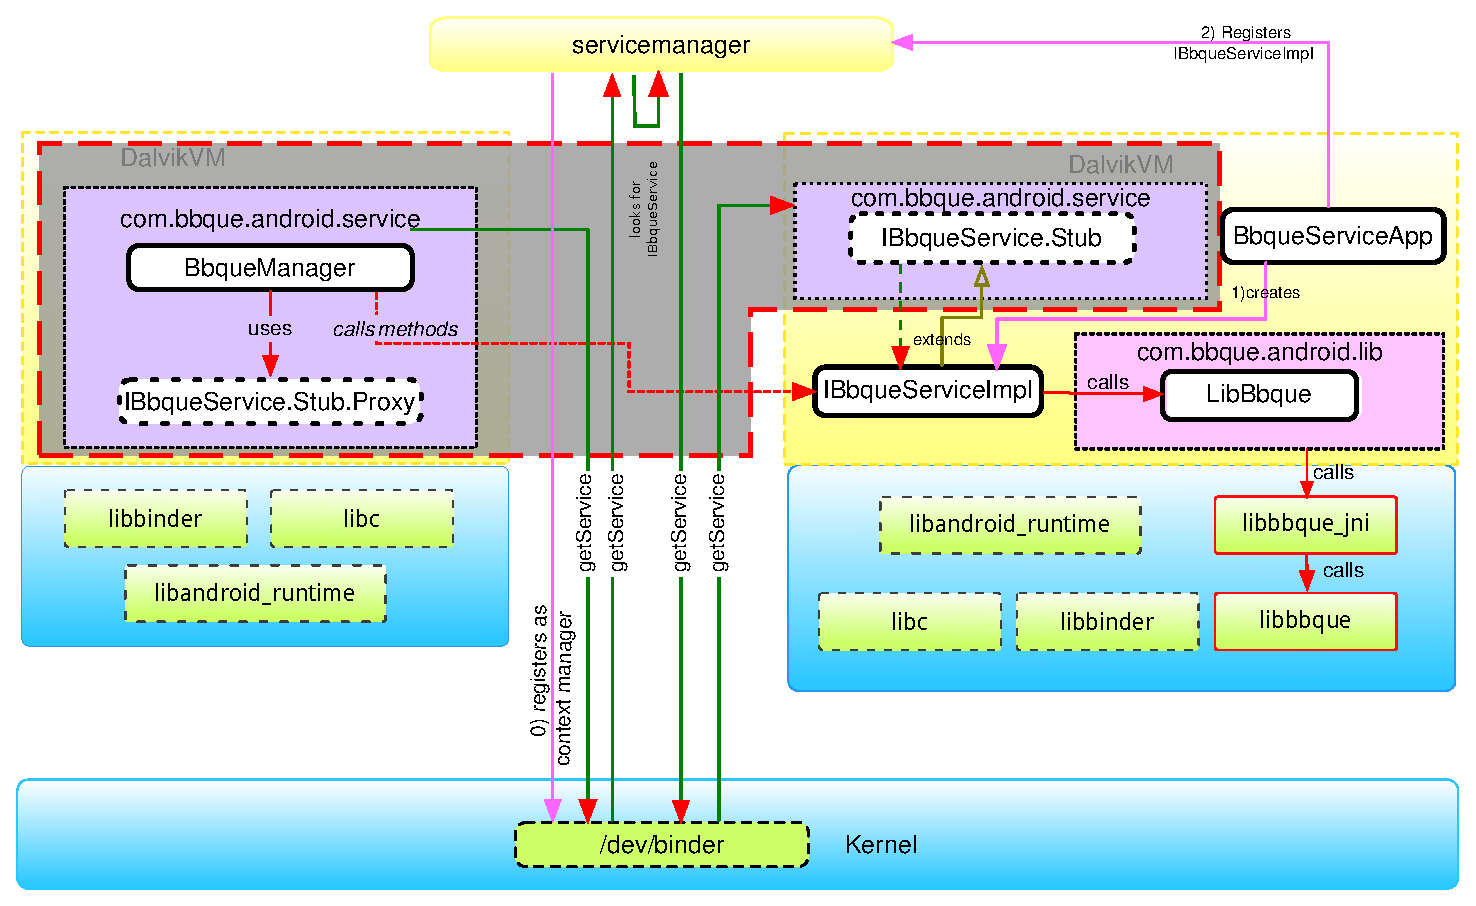
\includegraphics[scale=.505]{images/project_overview_binder.pdf}
	\caption{Interface-Library through binder}
	\label{fig:projectoverview_binder}
\end{figure}
\definecolor{lightgray}{gray}{0.93}
  \par\noindent\colorbox{lightgray}{%
    \begin{minipage}{0.98\textwidth}
		\textsc{RPC and Android Interface Definition Language}:\\
		Into Android, we do not use the Binder mechanism directly. Instead, we "define and interact with interfaces using Android's Interface Definition Language (IDL).
Interface definitions are usually stored in an \texttt{.aidl} file and are processed by the aidl tool to generate the proper stubs and marshalling/unmarshalling code required to transfer
objects and data back and forth using the Binder mechanism." \cite{embandroid}
    \end{minipage}%
  }%
  \vskip\baselineskip%
The working directory for this part is \texttt{bosp/p2012-common/framework/} where a new folder to include the interface and its manager has to be created (e.g. \texttt{bbqueservice}).
\begin{verbatim}
bbqueservice/
|---Android.mk
|---com/
|   |---bbque/
|       |---android/
|           |---service/
|               |---BbqueManager.java
|               |---IBbqueService.aidl
|---com.bbque.android.service.xml
\end{verbatim}
As seen for the previous module, \texttt{xml} file contains permissions declaration, and \texttt{Android.mk} file contains instructions for the building system to properly compile the module. Going deeper into folder's tree, there are two files:
\begin{itemize}
	\item \texttt{IBbqueService.aidl}\\
		As stated in the grey-coloured note above, this interface contains the methods' definitions. An example for our testing case is
		\begin{verbatim}
			interface IBbqueService {
			   int getNumCore();
			   [...]
			}
		\end{verbatim}
	\item \texttt{BbqueManager.java}\\
	This class is a proxy to our bounded service, and will be instantiated by any Application that will need to access to the Interface. It mainly returns the interface to the caller, as follows:
	\begin{verbatim}
		[...]
		import android.os.IBinder;
		import android.os.ServiceManager;
		[...]
		private final IBbqueService service;
		this.service = IBbqueService.Stub.asInterface(
		               ServiceManager.getService(REMOTE_SERVICE_NAME));
		[...]
	\end{verbatim}
\end{itemize}
\subsection{ServiceManager registering and Interface implementation}
Regarding the previous lines, to let the \texttt{BbqueManager} get the desired service, by calling the \texttt{ServiceManager.getService(...)} method, we must register our service into the Service Manager, otherwise it can't find - and therefore return - it to the caller. This operation is performed by a class called \texttt{BbqueServiceApp}. In Fig.\ref{fig:projectoverview_serviceapp} a portion of Fig.\ref{fig:projectoverview} focusing on this part can be seen.
\begin{figure}[!htb]
	\centering
	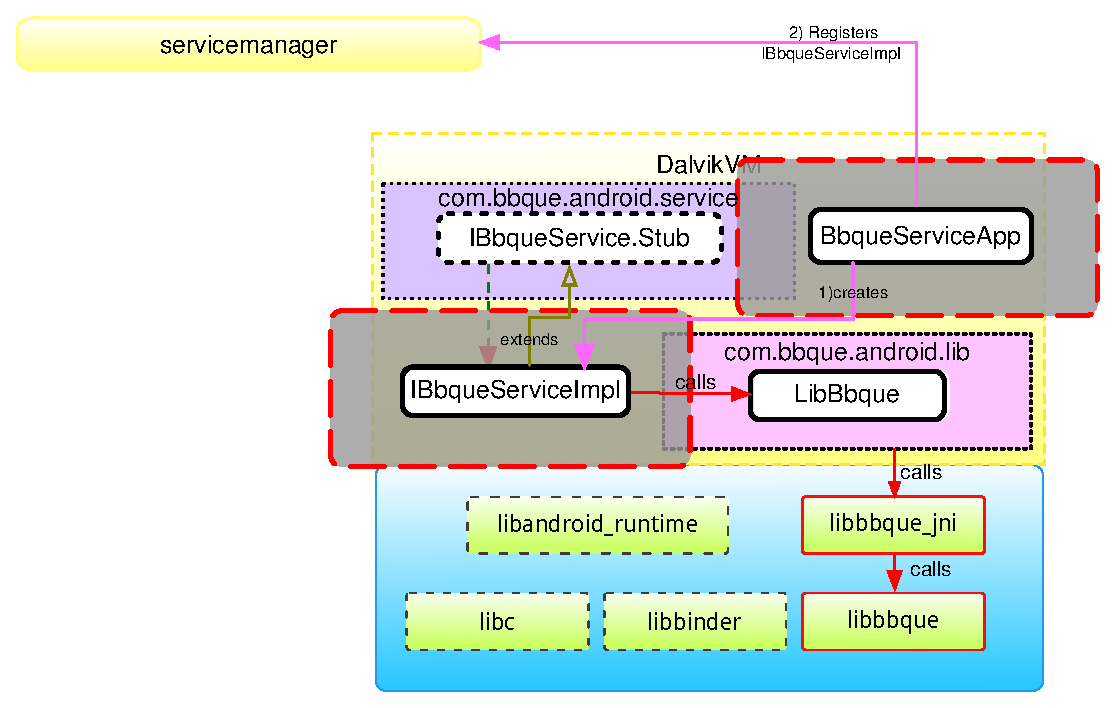
\includegraphics[scale=.505]{images/project_overview_IServiceImpl.pdf}
	\caption{Interaction ServiceApp - ServiceManager}
	\label{fig:projectoverview_serviceapp}
\end{figure}
The working directory is \texttt{bosp/p2012-common/app/}. Follows a tree summary within this folder.
\begin{verbatim}
app/
|---Android.mk
|---BbqueService
    |---AndroidManifest.xml
    |---Android.mk
    |---src
        |---com
            |---bbque
                |---android
                    |---bbqueservice
                        |---BbqueServiceApp.java
                        |---IBbqueServiceImpl.java
\end{verbatim}
\texttt{AndroidManifest.xml} file contains the declarations of the server application.\\
The inner \texttt{BbqueServiceApp.java} class, is declared as
\begin{verbatim}
public class BbqueServiceApp extends Application
\end{verbatim}
and \textit{overloads} the \texttt{onLoad} inherited method, with the \texttt{IBbqueServiceImpl} object creation, and its registration to the ServiceManager (pink arrows in Fig.\ref{fig:projectoverview_serviceapp}).
\begin{verbatim}
this.serviceImpl = new IBbqueServiceImpl(this);
ServiceManager.addService(REMOTE_SERVICE_NAME, this.serviceImpl);
\end{verbatim}
The \texttt{IBbqueServiceImpl.java} class, is declared as
\begin{verbatim}
class IBbqueServiceImpl extends IBbqueService.Stub
\end{verbatim}
and defines a constructor which takes as input a \texttt{Context} variable, and a simple \texttt{return} statement for each desired method we want to expose.\\
Finally, the last step before another building process, is to add this package to the main \textit{makefile} that, in our case, is \texttt{p2012-common/bosp\_p2012.mk}:
\begin{verbatim}
PRODUCT_PACKAGES += BbqueService
\end{verbatim}
As already seen before, the \texttt{+=} symbol, appends this last definition to all the others, to contribute to the creation of the main \textit{makefile}.\\
Android's log, during the startup, shows the following lines:
\begin{verbatim}
I/ActivityManager(  147): Start proc com.bbque.android.bbqueservice
               for added application com.bbque.android.bbqueservice:
               pid=242 uid=1000 gids={1015, 3002, 3001, 3003, 1028}
               
D/BbqueServiceApp(  242): Registered 
               [com.bbque.android.bbqueservice.IBbqueServiceImpl] as
               [com.bbque.android.service.IBbqueService]
\end{verbatim}
\subsection{Application layer}
\label{appLayer}
At this phase, everything is ready to be used by any Android Application/Activity. In Fig.\ref{fig:screenshot} a very simple application made to test the calls' flow, and in Fig.\ref{fig:shell} the \texttt{\$ adb logcat} output for a \texttt{get\_core\_availability()} call.
\begin{figure}[!htb]
	\centering
	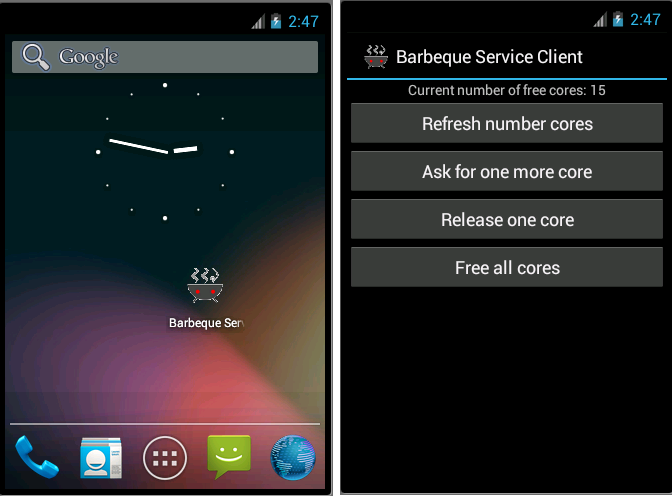
\includegraphics[scale=.505]{images/screenshot_duo.png}
	\caption{Home screen (left), Sample app (right)}
	\label{fig:screenshot}
\end{figure}
\begin{figure}[!htb]
	\centering
	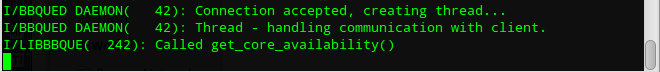
\includegraphics[scale=.505]{images/shell.png}
	\caption{Shell - Straight call}
	\label{fig:shell}
\end{figure}
\subsection{The other way around - callback}
\label{callbackSection}
If we wanted to see an example of how a similar call can go the opposite direction, we should implement a C-to-Java callback paradigm.\\
As long as I've seen, to achieve this result, the \textit{callback} approach requires - as the word itself clearly suggests - a first call from Java to C. Doing so, Java will pass to the native code (as previously seen in \ref{JNIwrapping}) some parameters as \texttt{JNIEnv} and \texttt{jclass}. Through these pointers, and some convenient specific functions, the native code is able to \textit{callback} a method coded within the Java class that made the first call: as long as the native process can hold the proper references to JNIEnv (or, actually, the global JavaVM, from which it can get back the environment) it will be able to make asynchronous calls to the Java methods belonging to the caller.\\
We'll briefly see the code used to achieve this which, at the moment of this writing, is contained into the Git \texttt{jb-callback} branch.
\begin{enumerate}
	\item The Java library \texttt{LibBbque} class (seen in \ref{JNIwrapping}) contains the following methods:
	\begin{verbatim}
		public native static int sendMessageToApp();
		
		public static void appCallback() {
		   System.out.println("JNI works.");
		}
	\end{verbatim}
	The former is needed to call the native library, and pass it the JNI parameters, while the latter is the class' method that C library will execute.
	\item As done before, after a \texttt{make} command, the JNI header file will be generated through a \texttt{javah -jni [...]} command. The result is
	\begin{verbatim}
		/*
		 * Class:     com_bbque_android_lib_LibBbque
		 * Method:    sendMessageToApp
		 * Signature: ()I
		 */
		 
		JNIEXPORT jint JNICALL
		          Java_com_bbque_android_lib_LibBbque_sendMessageToApp
		          (JNIEnv *, jclass);
	\end{verbatim}
	Its implementation will include the C native library, and call the native function:
	\begin{verbatim}
		#include <libbbque.h>
		#include "com_bbque_android_lib_LibBbque.h"
		[...]
		JNIEXPORT jint JNICALL
		          Java_com_bbque_android_lib_LibBbque_sendMessageToApp
		          (JNIEnv *env, jclass clazz) {
		             jint result = send_message_to_app(env, clazz);
		          [...]
		          }
	\end{verbatim}
	\item The callback implementation is mainly coded into this last native piece of code: the native library, \texttt{libbbque.c}
	\begin{verbatim}
		extern int send_message_to_app(JNIEnv *env, jclass clazz) {
		  __android_log_write(ANDROID_LOG_INFO, LOG_TAG,
		                      "Called send_message_to_app()");
		  jmethodID mid = (*env)->GetStaticMethodID (env, 
		                                             clazz,
		                                             "appCallback",
		                                             "()V");
		  (*env)->CallStaticVoidMethod(env, clazz, mid);
		  __android_log_write(ANDROID_LOG_DEBUG, LOG_TAG,
		                      "...method called back!");	
		  return 0;
		}
	\end{verbatim}
	This code allows a synchronous one-shot callback: the \texttt{GetStaticMethodId} looks for the \texttt{appCallback} method, with \texttt{()V} signature into the caller class: this means it will search for a \texttt{static void appCallback()} method. Its output fill be saved to \texttt{jmethodID} variable. This variable will be given as input parameter to the \texttt{CallStaticVoidMethod} method, to execute the callback.
	\item To test this implementation, we can let the Activity call the Java method which \textit{"opens"} the communication with C native library, by sending down the stack its JNIEnv and jclass data, as follows:
	\begin{verbatim}
		 public void run() {
		   [...]
		   this.bbqueManager.sendMessageToApp();
		 }
	\end{verbatim}
	The result of Activity launching, into the \texttt{catlog} screen is shown in Fig.\ref{fig:shell2}
\end{enumerate}
\begin{figure}[!htb]
	\centering
	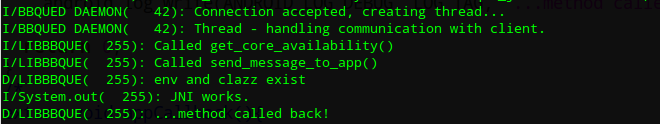
\includegraphics[scale=.505]{images/shell2.png}
	\caption{Shell - callback}
	\label{fig:shell2}
\end{figure}
The code of the native library could also save some global references (to be used asynchronously by any running process) as follows:
\begin{verbatim}
	//Saving GlobalJVM
	(*env)->GetJavaVM(env, &global_jvm);
	//Saving GlobalClass
	libbbque_global_class = (*env)->NewGlobalRef(env, clazz);
\end{verbatim}
These references should be passed to any daemon or running process, for future use, before the library loses them. This passage hasn't been implemented.

\bibliographystyle{acmtrans}
\bibliography{myrefs}
\nocite{embandroid}
\nocite{andinternals}
\nocite{opersys}
\nocite{learningandroid}
\nocite{jni}
\nocite{oracle}
\nocite{jnitips}
\nocite{smakov}

\begin{received}
August 20, 2012
\end{received}
\end{document}